%!TEX program = xelatex
\documentclass[9pt,dvipsnames,table]{beamer}
\usepackage[no-math,cm-default]{fontspec}
\usepackage[indentfirst]{xeCJK}
\usepackage{amsmath}
\usepackage{amsthm}
\usepackage{amssymb}
\usepackage{verbatim}
\usepackage{indentfirst}
\usepackage{syntonly}
\usepackage{beamerthemesplit}
\usepackage{ulem}
\usepackage{listings}
\usepackage{etoolbox}

\usetheme{Berlin}
\usecolortheme{beaver}
\usefonttheme[onlymath]{serif}
\CJKsetecglue{}
\setbeamerfont{section in toc}{size=\fontsize{10pt}{\baselineskip}}

%\setbeamerfont{normal text}{size=9pt}

\setCJKmainfont[BoldFont={SimHei},ItalicFont={KaiTi}]{SimSun}
\setmonofont[Scale=1]{Courier New}

\newcommand{\hlink}[1]{
	\footnote{\fontsize{6pt}{\baselineskip}\href{#1}{\textsl{\underline{#1}}}}
}
\newcommand{\image}[4]
{\begin{figure}[h]
	\centering
	\includegraphics[width=#3 \textwidth]{image/#2}
	\caption{#4}\label{#1}
\end{figure}}
\newcommand{\graph}[2]
{\begin{figure}[h]
	\centering
	\includegraphics[width=#2 \textwidth]{image/#1}
\end{figure}}
\newcommand{\graphold}[2]
{\begin{figure}[h]
	\centering
	\includegraphics[width=#1]{image/#2}
\end{figure}}

\lstset{language=C++,
	extendedchars=false,
	basicstyle=\ttfamily\footnotesize,
	keywordstyle=\bfseries\color{blue},
	identifierstyle=\color{blue!60!black},
	commentstyle=\itshape\color{gray},
	escapeinside=`'}

\setlength{\parindent}{2em}
\setlength{\baselineskip}{1.3\baselineskip}

\setbeamercolor{math text}{fg=black}
\setbeamertemplate{qed symbol}{$\square$}
\setbeamerfont{headline}{size=\fontsize{7.5pt}{\baselineskip}}
\setbeamerfont{footline}{size=\fontsize{7.5pt}{\baselineskip}}
\setbeamertemplate{theorems}[numbered]
\renewcommand{\thetheorem}{\arabic{subsubsection}.\arabic{theorem}}
\renewcommand{\thelemma}{\arabic{subsubsection}.\arabic{lemma}}
\newenvironment{qedframe}{%
	\begin{frame}[environment=qedqedframe]%
	}{%
	\qed
	\end{frame}%
}
\renewcommand{\appendixname}{结语}

\makeatletter
\patchcmd{\beamer@sectionintoc}{\vskip1.5em}{\vskip1em}{}{}
\makeatother

\begin{document}

\title[网络流]{\fontsize{24pt}{\baselineskip}网络流}
\subtitle[模型与例题]{\fontsize{16pt}{\baselineskip}模型与例题}
\author{清华大学计算机系~~胡泽聪}
%\institute[清华大学计算机系~~胡泽聪]{}
\date{}

\maketitle

%\setcounter{tocdepth}{1}
\begin{frame}
	\frametitle{目录}
	\tableofcontents[hideallsubsections]
\end{frame}

\section{前言}
\subsection{}
\begin{frame}
	\frametitle{预备知识}
	为了能听懂下面的题,你需要:
	\begin{itemize}
		\item 了解网络流模型的定义与含义。\pause
		\item 熟悉至少一种求网络流最大流的算法。如Dinic或者SAP。\pause
		\item 熟悉至少一种求费用流最小费用最大流的算法。如连续最短路算法或者ZKW改进版费用流。
	\end{itemize}
\end{frame}
\begin{frame}
	\frametitle{一些定义}
	\begin{itemize}
		\item $x\rightarrow y:w$代表从$x$到$y$容量为$w$的边。
		\item $x\rightarrow y:w,c$代表这条边有$c$的费用。
		\item $x\rightarrow y:[l,r]$代表这条边下界为$l$上界为$r$。
		\item $S$代表源点,$T$代表汇点。
	\end{itemize}
	
	由于网络流和费用流的算法基本上是固定的,故如非必要,则不会写出题目的数据范围。
\end{frame}
\begin{frame}
	\frametitle{常用方法}
	\begin{itemize}
		\item 增设源点汇点。
		\item 增设超级源点超级汇点。
		\item 拆点限流。
		\item 拆点表出入。
		\item ……
	\end{itemize}
\end{frame}

\section[Model I]{流量表示变迁}
\subsection{}
\begin{frame}
	\frametitle{流量表示变迁}
	最直观的应用。
	
	用流量表示事物的变迁。
	
	例如,某条路上走过了多少人,某个仓库流入流出的物品量,等等。\pause
	
	也可以说是流量代表一种方案。
\end{frame}

\subsection{POJ2391}
\begin{frame}
	\frametitle{Ombrophobic Bovines\hlink{http://poj.org/problem?id=2391} - 题意}
	给定一张的无向图,每条边有长度。点$i$处有$a_i$头牛,以及一个能容纳$b_i$头牛的牛棚。牛可以沿边移动,每条边上可以同时有任意头牛经过。一头牛经过一条边所需时间即为道路长度。
	
	给出一个将牛分配到牛棚的方案,并最小化所需移动时间$T$。
\end{frame}
\begin{frame}
	\frametitle{Ombrophobic Bovines - 模型}
	二分答案。\pause
	
	建立源点汇点。对每个点拆点,一个表示牛,一个表示牛棚。\pause
	
	对于一堆点,如果其最短路不超过二分的答案,则在其拆出的点之间连边,容量为无穷大。
	
	如果满流则可行。\pause
	
	不拆点会错。(想想为什么?)
\end{frame}

\subsection{POJ1149}
\begin{frame}
	\frametitle{PIGS\hlink{http://poj.org/problem?id=1149} - 题意}
	有$m$个猪圈,每个猪圈里初始时有若干头猪。一开始所有猪圈都是关闭的。
	
	依次来了$n$个顾客,每个顾客分别会打开指定的几个猪圈,从中买若干头猪。
	
	每个顾客分别都有他能够买的数量的上限。
	
	每个顾客走后,他打开的那些猪圈中的猪,都可以被任意地调换到其它开着的猪圈里,然后所有猪圈重新关上。
	
	问最多总共能卖出多少头猪。
	
	$1 \leq m \leq 1000$、$1 \leq n \leq 100$。
\end{frame}
\begin{frame}
	\frametitle{PIGS - 模型}
	先考虑朴素的模型。
	
	一共有$n$轮交易,那么我们建$n$排点,每排$m$个,代表每轮交易之前的猪圈。再对$n$个顾客设点。\pause
	
	对于每个顾客,向汇连边,容量为购买上限。
	
	源向第一轮的猪圈连边,容量为初始的数量。\pause
	
	对于第$i$个顾客能打开的猪圈,从第$i$轮的这些猪圈向该顾客连边,容量为无穷大。同时向第$i+1$轮的这些猪圈连边,容量同样为无穷大。
	
	点数为$O(nm)$。
\end{frame}
\begin{frame}
	\frametitle{PIGS - 模型}
	分开考虑每个猪圈。考虑能对其产生影响的若干顾客。
	
	只有这些顾客才能买,也只有他们才能移动猪圈里的猪。\pause
	
	那么从源向每个猪圈的第一个顾客连边,容量为初始的数量。
	
	每个猪圈的第$i$个顾客向第$i+1$个顾客连边,容量为无穷大。
	
	易知两模型等价。
\end{frame}

\subsection{POJ3281}
\begin{frame}
	\frametitle{Dining\hlink{http://poj.org/problem?id=3281} - 题意}
	有$a$种食物和$b$种饮料,每种食物或饮料只能供一头牛享用,且每头牛只享用一种食物和一种饮料。
	
	现在有$n$头牛,每头牛都有自己喜欢的食物种类列表和饮料种类列表。
	
	问最多能使几头牛同时享用到自己喜欢的食物和饮料。
\end{frame}
\begin{frame}
	\frametitle{Dining - 模型}
	如果只有食物,那这就是一个二分图匹配。\pause
	
	考虑一次增广,我们会选择一头牛、一种食物和一种饮料。
	
	那么我们设三排点,分别代表食物、牛和饮料。
	
	喜欢的食物$\rightarrow$牛$:1$,牛$\rightarrow$喜欢的饮料$:1$。
	
	$S\rightarrow$食物$:1$,饮料$\rightarrow T:1$。 \pause
	
	看似正确,实则错误。
	
	需要对牛拆点限流。
\end{frame}

\section[Model II]{最小割}
\subsection{}
\begin{frame}
	\frametitle{最小割}
	直观的应用,不好归进下面的分类中。反倒比较少见。
	
	一般来说要使得两边断开的东西都是最小割。
	
	可以有一些很厉害的应用。
\end{frame}

\subsection{<Unknown source>}
\begin{frame}
	\frametitle{Escape - 题意}
	有一条山谷,长度为$W$,宽度为$L$。有$n$个哨兵,第$i$个哨兵的视野为以其位置为圆心半径为$r_i$的圆。
	
	现在需要从山谷的最左侧走到最右侧而不进入任意一个哨兵的视野。问最少需要提前解决掉多少个哨兵。
	
	\graph{escape.png}{0.35}
\end{frame}
\begin{frame}
	\frametitle{Escape - 模型}
	这货还能绕弯走……我们或许得绕开传统的思路。\pause
	
	实际上,有一条路径等价于,山谷没有被``封死'',不会有视野横断了山谷的宽。\pause
	\vskip 1em
	我们对哨兵建两个点,之间连上容量为1的边,用来限流。
	
	设山谷的下边界为源,上边界为汇。
	
	对于两个哨兵,如果他们的视野相交,从左下的兵连向右上的兵,边权为无穷大。(对吗?)
	
	对于视野碰到了边界的,从源或向汇连边。\pause
	\vskip 1em
	实际上,我们应当从哨兵的入点连向出点。
	
	最小割就是答案。
\end{frame}

\subsection{BZOJ2561}
\begin{frame}
	\frametitle{最小生成树\hlink{http://www.lydsy.com/JudgeOnline/problem.php?id=2561} - 题意}
	一张$n$个点$m$条边的图,每条边有边权。
	
	现在在点$u$和点$v$之间加入一条权值为$L$的边。我们要使这条边既能出现在最小生成树上,又能出现在最大生成树上。
	
	问要满足这一条件,至少需要删去多少条边。
\end{frame}
\begin{frame}
	\frametitle{最小生成树 - 模型}
	生成树和最小割有什么关系?\pause
	
	最大生成树和最小生成树的边之间又有什么关系?\pause
	\vskip 1em
	考虑Kruskal算法。
	
	为了使加入的边能出现在最小生成树上而删去的边,与为了使加入的边能出现在最大生成树上而删去的边,一定不会不重复。\pause
	
	求最小生成树时,边权小于$L$的边在这条边加入前,不能使得$u$和$v$连通。最大生成树类似。\pause
	
	即为两边的最小割之和。
\end{frame}

\section[Model III]{最大权闭合子图}
\subsection{}
\begin{frame}
	\frametitle{最大权闭合子图}
	通常用来描述有依赖关系的若干物品的选择与否。其本质上是最小割。
	
	假设有$n$个物品,每个有自己的收益。收益可以为负。\pause
	
	视从$S$可达的点为选择,可达$T$的点为不选择。
	
	$S\rightarrow$收益为正的物品$:$收益,收益为负的物品$\rightarrow T:$收益的绝对值。
	
	如果$a$依赖于$b$,那么$b\rightarrow a:\infty$。
	
	答案为所有收益为正的物品的收益之和减去最小割。\pause
	
	正确性证明:\underline{\textbf{考虑一条增广路}}。
\end{frame}

\subsection{NOI2006}
\begin{frame}
	\frametitle{最大获利\hlink{http://www.lydsy.com/JudgeOnline/problem.php?id=1497} - 题意}
	有$n$个中转站的选址,在第$i$个地址处建造中转站的代价为$p_i$。
	
	有$m$个用户,第$i$个会在第$a_i$和$b_i$个中转站之间通讯,用户愿意支付$c_i$。
	
	求建造方案,使得获利最大。
\end{frame}
\begin{frame}
	\frametitle{最大获利 - 模型}
	作为网络流在NOI中的第一次亮相,难度还是非常平易近人的。
	
	就是最大权闭合子图的直接应用。\pause
	\vskip 1em
	将用户和中转站都视为物品,中转站收益为负,用户收益为正。
	
	用户依赖于相应两个中转站。
\end{frame}

\subsection{CEOI2008}
\begin{frame}
	\frametitle{Order - 题意}
	有$n$个项目和$m$台机器,每个项目依赖于一些机器。
	
	项目有正的收益。机器可以买,也可以租,都有各自的代价。借一次机器可以给一个项目用一次。
	
	求最大收益。
\end{frame}
\begin{frame}
	\frametitle{Order - 模型}
	如果机器不能借,那么就是最经典的最大权闭合子图。\pause
	\vskip 1em
	这个题目的难点在于机器可以借。
	
	我们先按照最大权闭合子图的模型建图。考虑一条增广路,一定是$S\rightarrow$项目$\rightarrow$机器$\rightarrow T$。
	
	割第一条边是放弃项目,割第三条边是买机器。第二条边是无穷大。\pause
	
	如果我们设割第二条边是租机器呢?把无穷大改为租用费用。
	
	答案是项目收益之和减去最小割。
\end{frame}

\subsection{Codeforces Round \#185 (Div. 1) - E}
\begin{frame}
	\frametitle{Biologist\hlink{http://codeforces.com/contest/311/problem/E} - 题意}
	有$n$个点,每个可以是白色或者黑色。可以花$v_i$的代价改变第$i$个点的颜色。
	
	有$m$条件,每个条件都是要求某一些点都是某种颜色。如果满足了第$i$个条件可以得到$g_i$的收益,没有满足则须付出$l_i$的代价。
	
	求最大收益。
\end{frame}
\begin{frame}
	\frametitle{Biologist - 模型}
	没有条件的话,也就是经典模型了。
	
	白点$\rightarrow T:$代价,$S\rightarrow$黑点$:$代价。\pause
	
	我们可以也对条件建点。
	
	如果条件是都是黑色,$S\rightarrow$条件$:$收益+代价。条件$\rightarrow$点$:\infty$。
	
	如果条件是都是白色,条件$\rightarrow T:$收益+代价。点$\rightarrow$条件$:\infty$。
	
	正确性证明同样考虑增广路。
\end{frame}

\subsection{一类经典问题}
\begin{frame}
	\frametitle{二元费用问题 - 题意}
	有$n$个点,选和不选各自有收益。有$m$个条件,有三种:
	\begin{itemize}
		\item 如果$x$和$y$都选了,获得$w$的收益;
		\item 如果$x$和$y$都没选,获得$w$的收益;
		\item 如果$x$和$y$都一个选了一个没选,付出$w$的代价。
	\end{itemize}
	
	求最大收益。
\end{frame}
\begin{frame}
	\frametitle{二元费用问题 - 模型}
	我们用类似最大权闭合子图的方法建图。
	
	只考虑有关系的两个点,可以得出长成下面这个样子的东西。
	
	\graph{cost.png}{0.5}
	
	我们的目标是确定$S_x$、$S_y$、$T_x$、$T_y$和$w$的值。
\end{frame}
\begin{frame}
	\frametitle{二元费用问题 - 模型}
	设选$x$的收益为$VA_x$,不选的是$VB_x$,$x$和$y$都选的收益为$EA$,都不选的收益为$EB$,一选一不选的代价为$EC$。\pause
	
	考虑每种情况:
	\begin{itemize}
		\item $x$和$y$都选。此时被割的边为$S_x+S_y$。
		\item $x$和$y$都没选。此时被割的边为$T_x+T_y$。
		\item $x$选$y$没选。此时被割的边为$S_x+T_y+w1$。
		\item $x$没选$y$选。此时被割的边为$T_x+S_y+w2$。
	\end{itemize}
\end{frame}
\begin{frame}
	\frametitle{二元费用问题 - 模型}
	我们知道被割的边是损失掉的代价。所以有
	\begin{eqnarray*}
		S_x+S_y & = & VB_x+VB_y+EB \\
		T_x+T_y & = & VA_x+VA_y+EA \\
		S_x+T_y+w1 & = & VB_x+VA_y+EA+EB+EC \\
		T_x+S_y+w2 & = & VA_x+VB_y+EA+EB+EC \\
		w1 & = & w2
	\end{eqnarray*}
	其中最后一个是我们的假设。\pause

	这个方程组的自变量多于方程数,有无穷组解。
\end{frame}
\begin{frame}
	\frametitle{二元费用问题 - 模型}
	下面是其中一组解:
	\begin{eqnarray*}
		S_x & = & VB_x+\frac{EB}{2} \\
		T_x & = & VA_x+\frac{EA}{2} \\
		w1=w2 & = & \frac{EA+EB}{2}+EC
	\end{eqnarray*}
	
	答案即$\sum{VA+VB+EA+EB}$减去最小割。为避免小数可以给所有权值乘以2。
\end{frame}

\section[Model IV]{平面图对偶图}
\subsection{}
\begin{frame}
	\frametitle{平面图对偶图}
	\begin{columns}
		\begin{column}{0.45\textwidth}
			\uncover<1->{什么是平面图?}
			\vskip 0.5em
			\uncover<2->{什么是平面图的对偶图?}
			\vskip 0.5em
			\uncover<3->{如何构造平面图的对偶图?}
			\vskip 0.5em
			\uncover<5->{如何把问题转换到对偶图上?}
			\vskip 0.5em
			\uncover<6->{为何要使用对偶图来求解?}
		\end{column}
		\begin{column}{0.45\textwidth}
			\uncover<4->{\graph{planar.png}{1.0}}
		\end{column}
	\end{columns}
\end{frame}

\subsection{BeiJing2006 (BZOJ1001)}
\begin{frame}
	\frametitle{狼抓兔子\hlink{http://www.lydsy.com/JudgeOnline/problem.php?id=1001} - 题意}
	\graph{1001.png}{0.55}
	
	$n\times m$的类似网格的图,如上所示。求从``START''到``END''的最小割。
	
	$n,m\leq 1000$。
\end{frame}
\begin{frame}
	\frametitle{狼抓兔子 - 模型}
	数据范围很大,直接做网络流会超时。
	
	故转换成对偶图上的最短路。
\end{frame}

\subsection{NOI2010 (BZOJ2007)}
\begin{frame}
	\frametitle{海拔\hlink{http://www.lydsy.com/JudgeOnline/problem.php?id=2007} - 题意}
	\begin{columns}
		\begin{column}{0.475\textwidth}
			  $n\times n$的网格图,每条边双向通行。已知每条边两个方向的人流量,你需要给每个点$x$设定海拔高度$h_x$。左上角的高度为0,右下角的高度为1。对于$x$到$y$的流量为$w$的边,代价为$w\times\max(0,h_y-h_x)$。求最小代价。
			
			  $n\leq 500$。
		\end{column}
		\begin{column}{0.45\textwidth}
			\graph{2007_1.png}{1.0}
		\end{column}
	\end{columns}
\end{frame}
\begin{frame}
	\frametitle{海拔 - 模型}
	\begin{columns}
		\begin{column}{0.475\textwidth} \pause
			\begin{itemize}
				\item[结论1] 每个点的海拔非0即1。\pause
			
				\item[结论2] 海拔为0的点构成一个连通块,海拔为1的点亦同。\pause
			\end{itemize}
			\vskip 1em
			  其实就是求左上角和右下角的最小割。转换成对偶图上的最短路。
			
			  边的方向呢?\pause
		\end{column}
		\begin{column}{0.45\textwidth}
			\graph{2007_2.png}{1.0}
		\end{column}
	\end{columns}
\end{frame}

\subsection{Codejam Round 2 2014 C}
\begin{frame}
	\frametitle{Don't Break The Nile\hlink{https://code.google.com/codejam/contest/3014486/dashboard\#s=p2\&a=2} - 题意}
	\begin{columns}
		\begin{column}{0.475\textwidth}
			  $n\times m$的网格图,底部的每个格子接受1的入流量,顶部的每个格子可以流出1的流量,每个格子可以流过1的流量。图中有$k$个长方形区域是不能走流量的,这些长方形互不相交,但可以有公共边。求图的最大流。
			
			  $m\leq 1000$,$n\leq 10^8$,$k\leq 1000$。
		\end{column}
		\begin{column}{0.45\textwidth}
			\graph{codejam_1.png}{0.75}
		\end{column}
	\end{columns}
\end{frame}
\begin{frame}
	\frametitle{Don't Break The Nile - 模型}
	\begin{columns}
		\begin{column}{0.45\textwidth}
			  暴力怎么做?\pause 
			
			  需要拆点吗?\pause
			
			  虽然要,但考虑其最小割,割掉的一定是点内部的边。\pause
			
			  割掉内部边相当于把格子填成黑色。\pause
			
			  可以转换成河两岸之间的最短路问题,如右图。
		\end{column}
		\begin{column}{0.45\textwidth}
			\graph{codejam_2.png}{0.8}
		\end{column}
	\end{columns}
\end{frame}

\section[Model V]{费用递增}
\subsection{}
\begin{frame}
	\frametitle{费用递增}
	这类模型是一类费用流模型,它代表着某个东西可以选择若干次,而次数每加1所需要的代价是递增的。一种常见情况是选择$x$的代价为$x^2$。
\end{frame}
\subsection{JSOI2009 (BZOJ1449)}
\begin{frame}
	\frametitle{球队收益\hlink{http://www.lydsy.com/JudgeOnline/problem.php?id=1449} - 题意}
	有$n$支球队,有些球队之间已经打了一些比赛了,现给出每个球队的数据$win$、$lose$、$C$和$D$,分别表示已胜场数、已负场数,以及计算收益的两个系数。
	
	一支球队的收益为$Cw^2+Dl^2$,其中$w$和$l$是最后胜负的场数。接下来还有$m$场比赛。给出接下来$m$场比赛的对阵情况,求出$n$支球队收益和的最小值。接下来$m$场比赛的胜负是你可以决定的。
\end{frame}
\begin{frame}
	\frametitle{球队收益 - 模型}
	应该可以想到是费用流模型,关键在于建模。\pause
	\vskip 1em
	一场比赛必然有一个赢家和一个输家,但是似乎不太好同时在模型中表示。不妨先假设后面的$m$场比赛中双方都是输家,这样我们只要在模型中表示一方成为赢家即可。\pause
	\vskip 1em
	至此应该有一个初步的模型了:对于$n$支球队和$m$场比赛各建一个点,从源向每场比赛连流量1费用0的边,从比赛向参与这场比赛的两支队伍各连一条流量1费用0的边。剩下的就是队伍收益的费用表示了。
\end{frame}
\begin{frame}
	\frametitle{球队收益 - 模型}
	我们考虑费用的增量:多赢一场比赛产生的收益。
	
	即$(C(w+1)^2+D(l-1)^2)-(Cw^2+Dl^2)=2wC-2lD+C+D$。\pause
	
	对于第$i$支队伍,假设后$m$场中$i$参加的有$x$场,那么最初$w=win,$ $l=lose+x$,之后每赢一场$w$加一,$l$减一。我们从第$i$支队伍的点向汇连$x$条边,分别代表第$i$支队伍赢了$j$场比赛时相对赢$j-1$场时收益的增量。由于增量一定越来越大,所以流量最先流过的一定是费用较小的边,即$j$最小的边。\pause
	\vskip 1em
	至此模型完成,答案即所有队伍最初收益+最小费用最大流的费用。
\end{frame}

\subsection{SCOI2007 (BZOJ1070)}
\begin{frame}
	\frametitle{修车 - 题意}
	有$n$辆车和$m$名修理工,一名修理工在一个时刻只能修一辆车,并且在修完一辆之后才能开始修下一辆。已知每位修理工修每辆车的时间,求顾客的最小平均等待时间。顾客的等待时间为他的车被修好的时间。
\end{frame}
\begin{frame}
	\frametitle{修车 - 模型}
	所求即最小的总等待时间。假设已经确定了每辆车被谁修理,以及每个人修理的顺序,如何计算代价?\pause
	
	对于每个人分开算,如果一个人一共修理$k$辆车,那么修的第$i$辆车对于代价的贡献为$k-i+1$倍。
	
	此处费用递减,而且我们无法确定一共有多少车!怎么办?
\end{frame}
\begin{frame}
	\frametitle{修车 - 模型}
	倒着考虑。我们考虑一辆车是倒数第几个修的。
	
	对车和修理工的倒数第几个``修车位''设点,连边:
	
	车$\rightarrow$第$k$个修车位$:(k-i+1)$倍时间。
	
	最小费用最大流即为答案。
\end{frame}

\subsection{WC2007 (BZOJ2597)}
\begin{frame}
	\frametitle{剪刀石头布\hlink{http://www.lydsy.com/JudgeOnline/problem.php?id=2597} - 题意}
	有$n$个人,两两之间进行一次比赛。有些比赛已经进行了,有些还没有。我们用一个竞赛图来表示输赢情况,一场比赛的有向边从输家连向赢家。
	
	你可以决定尚未进行的比赛的输赢情况,使得下面这种三元组的数量最多:$(a,b,c)$表示一个无序三元组($(a,b,c)$的任意排列都算同一种),其中存在有向边$a\rightarrow b$、$b\rightarrow c$、$c\rightarrow a$。
	
	需要输出方案。$n\leq 100$。
\end{frame}
\begin{frame}
	\frametitle{剪刀石头布 - 模型}
	有种即视感?似乎和上面的题很像,但是这里的东西似乎更不好表示。不如我们先考虑,给定这样一个图,求这样的三元组的数目。\pause
	\vskip 1em
	从$n$个点中任选3个的方案数为$\binom{n}{3}$,考虑怎么样的三元组是不合法的:这样的三元组的导出子图中一定有一个点的入度为2。设第$i$个点的入度为$d_i$,那么不合法的三元组数为$\sum{\binom{d_i}{2}}$。所有合法方案为:
\end{frame}
\begin{frame}
	\frametitle{剪刀石头布 - 模型}
	\begin{eqnarray*}
		 & & \binom{n}{3}-\sum\binom{d_i}{2} \\
		 & = & \binom{n}{3}-\frac{1}{2}\sum(d_i(d_i-1)) \\
		 & = & \binom{n}{3}+\frac{1}{2}\sum{d_i}-\frac{1}{2}\sum{d_i^2}
	\end{eqnarray*}\pause
	
	注意$\sum{d_i}$是定值,就是$\binom{n}{2}$。那么剩下的就和上面那题一模一样了吧?至于输出方案,只要看比赛的点连出的边连向了哪个点即可。
\end{frame}

\section[Model VI]{流量平衡}
\subsection{}
\begin{frame}
	\frametitle{流量平衡}
	网络流模型中,除了源点和汇点以外,每个点都满足流量平衡条件。
	
	即,每个点流入的流量等于其流出的流量。
	
	利用这个性质来解决一些拥有类似性质的题目。
\end{frame}

\subsection{TCO2013 R1AL3 / BZOJ3171}
\begin{frame}
	\frametitle{DirectionBoard\hlink{http://www.lydsy.com/JudgeOnline/problem.php?id=3171} - 题意}
	一块$n\times m$的地图,每个格子内有一个箭头。
	
	从某个格子出发,沿着箭头的方向走,从一侧出了边界就从另一侧进入。
	
	如果从任意一个格子出发都能回到出发的格子,那么地图就是合法的。
	
	给定地图,求至少要改变几个格子的箭头的方向,才能使得地图合法。
	
	\graph{BZOJ3171.png}{0.35}
\end{frame}
\begin{frame}
	\frametitle{DirectionBoard - 模型}
	先考虑判断一个地图是否合法。\pause
	\vskip 1em
	把每个格子抽象成节点,向箭头指向的格子连边。
	
	每个格子可以沿箭头回到自己,等价于模型中的每个节点都在一个环中。
	
	而每个节点的出度为1,所以即图中每个连通块都是环。也即每个点的入度为1,出度为1。\pause
	
	也就是流量平衡。那么我们建立网络流模型,对每个点拆点成入点和出点。满流即合法。 \pause
	\vskip 1em
	考虑改变方向,我们可以花费代价搬迁连出去的边。\pause
	
	把网络流改成费用流,原有边的费用为0,每个格子的出点向相邻的非箭头所指格子的入点连一条费用为1的边。
\end{frame}

\subsection{SRM570 D1L3}
\begin{frame}
	\frametitle{CurvyonRails - 题意}
	一块$n\times n$的地图,每个格子均为空地或者障碍。 
	
	现在要铺铁轨,每块空地都要被覆盖,每条路线必须闭合,且不能相交。
	
	有些空地上住着弯星人,在这种空地上铺一块直的铁路需要花费1的代价。 
	
	给定地图,求是否能够铺铁轨,以及最小代价。
	
	{\noindent
	\begin{figure}[h!]
		\centering
		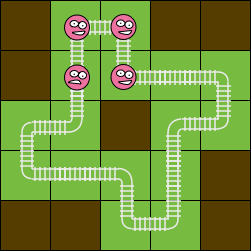
\includegraphics[width=2.5cm]{image/SRM570_1.png}
		\hskip 2em
		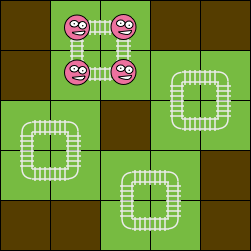
\includegraphics[width=2.5cm]{image/SRM570_2.png}
	\end{figure}
	}
\end{frame}
\begin{frame}
	\frametitle{CurvyonRails - 模型}
	先考虑判断是否有解。\pause
	
	有解即,存在一些不相交的回路可以覆盖所有空地且不覆盖任意障碍。
	
	也即,每个空地向相邻的空地连出恰好两条轨道。\pause
	\vskip 1em
	那么构建网络流模型。
	
	对空地黑白染色,从源向黑点、从白点向汇连容量为2的边。
	
	从黑点向相邻的白点连容量为1的边。满流即有解。
	
	\graphold{7cm}{SRM570_3.png}
\end{frame}
\begin{frame}
	\frametitle{CurvyonRails - 模型}
	那么弯的和直的铁轨怎么判断?\pause
	\vskip 1em
	直的铁轨即,一块空地连出两条横向或纵向的轨道。
	
	弯的铁轨即,一块空地连出一条横向和一条纵向的轨道。
	
	先强制所有铁轨都是弯的,判断是否有解。\pause
	\vskip 1em
	在已有的网络流模型基础上改进。
	
	把每块空地拆成两个点,一个代表横向,一个代表纵向。
	
	横向点向横向相邻的空地的横向点连一条容量为1的边,纵向的类似。满流即有解。
\end{frame}
\begin{frame}
	\frametitle{CurvyonRails - 模型}
	\graphold{4.5cm}{SRM570_4.png}
\end{frame}
\begin{frame}
	\frametitle{CurvyonRails - 模型}
	如果要把一块铁轨改成直的呢?
	
	如果是没人的空地,随便改;如果是有人的空地,收取费用。\pause
	\vskip 1em
	把网络流模型改成费用流模型,已有的边费用为0。
	
	在一块空地拆出的两个点之间连一条流量为1的双向边。
	
	如果空地有人,双向边的费用为1;否则为0。
	
	如果这类边有流量,就说明有一条轨道改变了方向。答案即为最小费用最大流。
\end{frame}
\begin{frame}
	\frametitle{CurvyonRails - 模型}
	\graphold{4.5cm}{SRM570_5.png}
\end{frame}
	
\appendix
\section{}
\begin{frame}
	\frametitle{Fin.}
	\centering
	\LARGE
	谢谢大家!欢迎课后交流。
\end{frame}

\end{document}
